\documentclass[12pt,letterpaper]{report}
\usepackage[margin=1in]{geometry}
\usepackage{titlesec}
\usepackage{amsmath}
\usepackage{amssymb}
\usepackage[colorlinks=true,urlcolor=black,linkcolor=black]{hyperref}
\usepackage{graphicx}
\usepackage{textcomp}
\graphicspath{ {./images/} }
% extra packages you need

\titleformat{\chapter}{\bf\huge}{\thechapter}{20pt}{\huge\vspace{-.5em}}

\begin{document}

\title{\begin{figure}[htb]
\begin{center}

\includegraphics[width=8cm]{univ_logo}
\end{center}
\end{figure}SOEN 6011 : SOFTWARE ENGINEERING PROCESSES\\[.5em]
SUMMER 2022\\\vspace*{0.9in}
\begin{Large}
\textbf{ETERNITY} 
\end{Large}
\vspace*{0.7in}
\begin{Large}
\textbf{\\PROBLEM - 5} 
\\Unit Test Cases\\
\small{https://github.com/PrathikaSuvarna/ScientificCalculator}
\end{Large}}
\author{By Prathika Anup Suvarna (40156790)}
\maketitle 
\pagenumbering{roman}
\setcounter{page}{0}

\tableofcontents


%%%%%%%%%%%%%%%%%%%%%%%%%%%%%%
\chapter{Unit Test Cases Description}
\pagenumbering{arabic}

\section{Test Environment}
\begin{enumerate}
\item IntelliJ IDE (2022) for Java.
\item JUnit4 framework in IntelliJ IDE for testing.
\end{enumerate}

\begin{center}
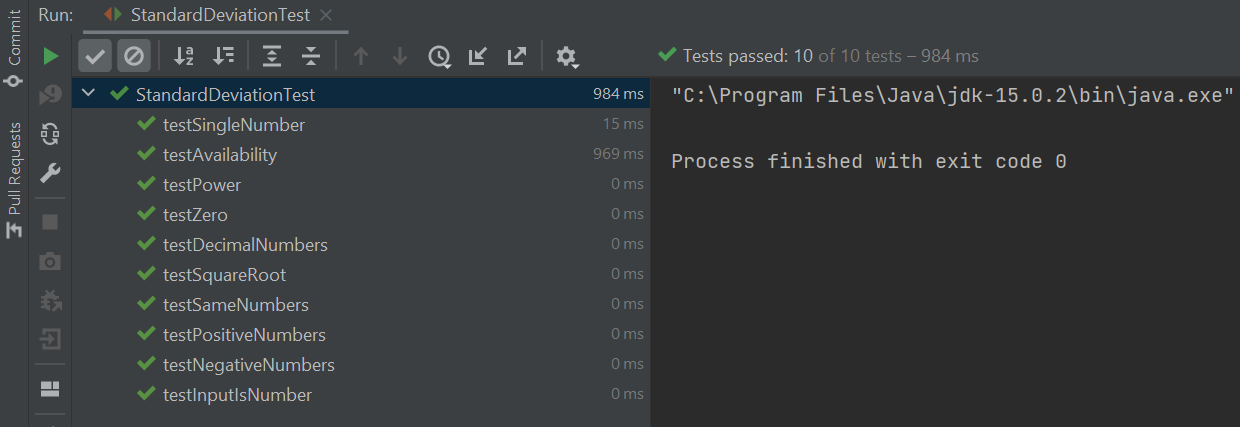
\includegraphics[width=15cm,height=6cm]{UnitTest}
\end{center}

\section{Descriptions}
\normalsize{The unit test cases for $\sigma$ function is done using Junit4 which is traceable to the \\requirements in Problem 2.}
\\\\\\
\textbf{Test Case : F8\_UnitTestCase\_1}\\\\
\begin{tabular}{ll}
\textbf{Test Case ID} & F8\_TestInputZero\\\\
\textbf{Requirement ID} & R1 \\
\textbf{Action} & 
\begin{tabular}[c]{@{}l@{}}The user gives an input 0 and
\\then clicks SD($\sigma$) button. \\
\end{tabular} \\
\textbf{Input(s) } & 0 \\
\textbf{Expected Output } & 0 \\
\textbf{Actual Output } &   0 \\
\textbf{Test Result } & Success \\
\end{tabular}
\\\\\\\\
\textbf{Test Case : F8\_UnitTestCase\_2}\\\\
\begin{tabular}{ll}
\textbf{Test Case ID} & F8\_TestSingleNumber\\\\
\textbf{Requirement ID} & R2 \\
\textbf{Action} & 
\begin{tabular}[c]{@{}l@{}}The user gives an input 5 and
\\then clicks SD($\sigma$) button. \\
\end{tabular} \\
\textbf{Input(s) } & 5 \\
\textbf{Expected Output } & 0 \\
\textbf{Actual Output } &   0 \\
\textbf{Test Result } & Success \\
\end{tabular}
\\\\\\\\
\textbf{Test Case : F8\_UnitTestCase\_3}\\\\
\begin{tabular}{ll}
\textbf{Test Case ID} & F8\_TestSameNumbers\\\
\textbf{Requirement ID} & R3\\
\textbf{Action} & 
\begin{tabular}[c]{@{}l@{}}The user gives an input [8 8 8 8 8] and
\\then clicks SD($\sigma$) button. \\
\end{tabular} \\
\textbf{Input(s) } & [8 8 8 8 8] \\
\textbf{Expected Output } & 0 \\
\textbf{Actual Output } &   0 \\
\textbf{Test Result } & Success \\
\end{tabular}
\\\\\\\\
\textbf{Test Case : F8\_UnitTestCase\_4}\\\\
\begin{tabular}{ll}
\textbf{Test Case ID} & F8\_TestNegativeNumbers\\\\
\textbf{Requirement ID} & R4 \\
\textbf{Action} & 
\begin{tabular}[c]{@{}l@{}}The user gives an input [-8 -6 9 -10 5] and
\\then clicks SD($\sigma$) button. \\
\end{tabular} \\
\textbf{Input(s) } & [-8 -6 9 -10 5] \\
\textbf{Expected Output } & 7.5630681604756 \\
\textbf{Actual Output } &   7.5630681604756 \\
\textbf{Test Result } & Success \\
\end{tabular}
\\\\\\\\
\textbf{Test Case : F8\_UnitTestCase\_5}\\\\
\begin{tabular}{ll}
\textbf{Test Case ID} & F8\_TestPositiveNumbers\\\\
\textbf{Requirement ID} & R5\\
\textbf{Action} & 
\begin{tabular}[c]{@{}l@{}}The user gives an input [8 6 9 10 5] and
\\then clicks SD($\sigma$) button. \\
\end{tabular} \\
\textbf{Input(s) } & [8 6 9 10 5] \\
\textbf{Expected Output } & 1.8547236990991407 \\
\textbf{Actual Output } &   1.8547236990991407 \\
\textbf{Test Result } & Success \\
\end{tabular}
\\\\\\\\
\textbf{Test Case : F8\_UnitTestCase\_6}\\\\
\begin{tabular}{ll}
\textbf{Test Case ID} & F8\_TestDecimalNumbers\\\\
\textbf{Requirement ID} & R6 \\
\textbf{Action} & 
\begin{tabular}[c]{@{}l@{}}The user gives an input [8.2 6.4 1.9 7.5 5] and
\\then clicks SD($\sigma$) button. \\
\end{tabular} \\
\textbf{Input(s) } & [8.2 6.4 1.9 7.5 5] \\
\textbf{Expected Output } & 2.2297981971472 \\
\textbf{Actual Output } &   2.2297981971472 \\
\textbf{Test Result } & Success \\
\end{tabular}
\\\\\\\\
\textbf{Test Case : F8\_UnitTestCase\_7}\\\\
\begin{tabular}{ll}
\textbf{Test Case ID} & F8\_TestSquareRoot\\\\
\textbf{Requirement ID} & R7\\
\textbf{Action} & 
\begin{tabular}[c]{@{}l@{}}Input 2 is given
to the $\sqrt{x}$ function. \\
\end{tabular} \\
\textbf{Input(s) } & 2 \\
\textbf{Expected Output } & 1.4142135623746899 \\
\textbf{Actual Output } &   1.4142135623746899\\
\textbf{Test Result } & Success \\
\end{tabular}
\\\\\\\\
\textbf{Test Case : F8\_UnitTestCase\_8}\\\\
\begin{tabular}{ll}
\textbf{Test Case ID} & F8\_TestPower\\\\
\textbf{Requirement ID} & R8 \\
\textbf{Action} & 
\begin{tabular}[c]{@{}l@{}} Input 5 as base and exponent 2 is given
\\to the power(x,y) function. \\
\end{tabular} \\
\textbf{Input(s) } & 5,2 \\
\textbf{Expected Output } & 25 \\
\textbf{Actual Output } &   25 \\
\textbf{Test Result } & Success \\
\end{tabular}
\\\\\\\\
\textbf{Test Case : F8\_UnitTestCase\_9}\\\\
\begin{tabular}{ll}
\textbf{Test Case ID} & F8\_TestInputisNumber\\\\
\textbf{Requirement ID} & R9 \\
\textbf{Action} & 
\begin{tabular}[c]{@{}l@{}}The user gives an input "g" and
then clicks SD($\sigma$) button. \\
\end{tabular} \\
\textbf{Input(s) } & "g" \\
\textbf{Expected Output } & false \\
\textbf{Actual Output } &   false \\
\textbf{Test Result } & Success \\
\end{tabular}
\\\\\\\\
\textbf{Test Case : F8\_UnitTestCase\_10}\\\\
\begin{tabular}{ll}
\textbf{Test Case ID} & F8\_TestAvailability\\\\
\textbf{Requirement ID} & R10 \\
\textbf{Action} & 
\begin{tabular}[c]{@{}l@{}}The user gives any input
then clicks SD($\sigma$) button. \\
\end{tabular} \\
\textbf{Input(s) } & Any real numbers \\
\textbf{Expected Output } & positive real number \\
\textbf{Actual Output } & positive real number \\
\textbf{Test Result } & Success \\
\end{tabular}
\\\\\\\\

\begin{thebibliography}{9}
    \addcontentsline{toc}{chapter}{Bibliography}

\bibitem{ReqView} 
ReqView : Nykamp DQ: Requirements Specification Templates
\\\texttt{https://www.reqview.com/doc/iso-iec-ieee-29148-templates}
\bibitem{29148} 
29148-2018-ISO/IEC/IEEE International Standard-Systems and software engineering-Life cycle processes-Requirements engineering,
\\\texttt{https://standards.ieee.org/standard/29148-2018.html}
\end{thebibliography}

\end{document}
